\documentclass{SKP-beamer}

% --------------------------------------------------- %
%                  Presentation info	              %
% --------------------------------------------------- %
\title[General Disease Prediction System]{Predicting the Unpredictable: A General Disease Forecasting System}
\subtitle{Ideation}
\author{Silicon Institute of Technology}
\institute[SBP]{
  DEPARTMENT OF COMPUTER SCIENCE AND ENGINEERING
}
\date{\today}
\logo{
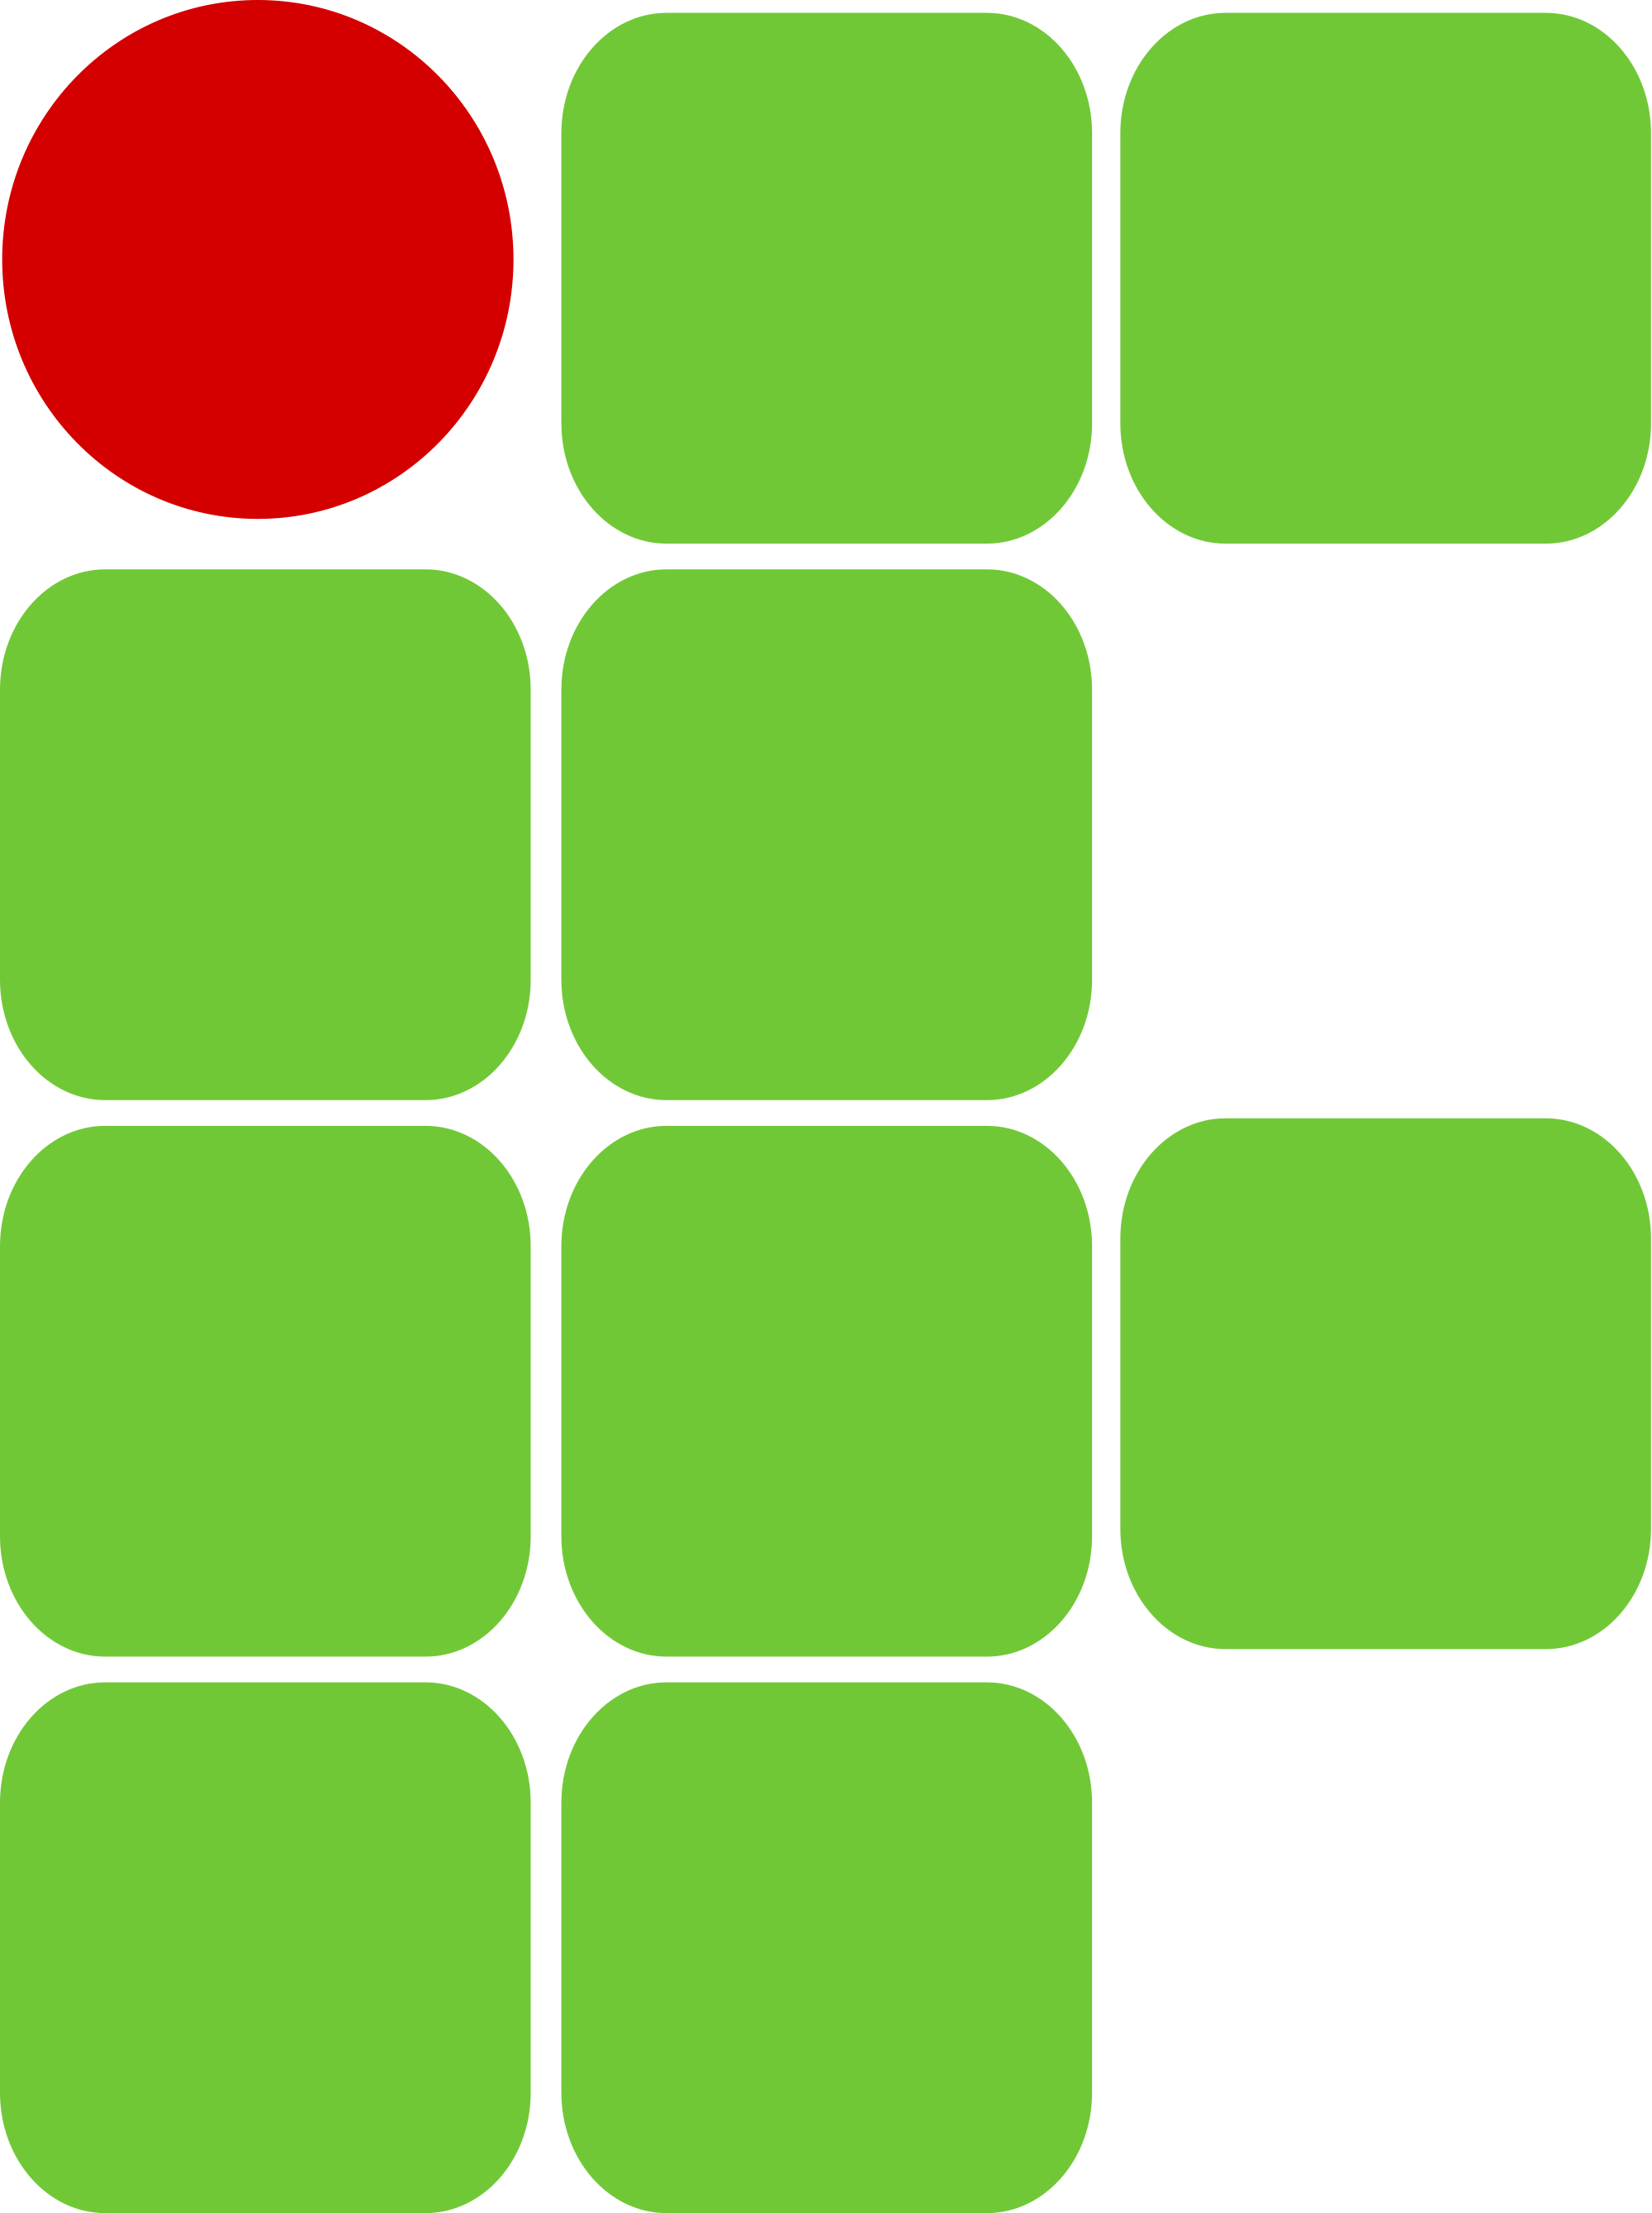
\includegraphics[scale=0.008]{images/logo.png}
}
\subject{Presentation subject} % metadata

% --------------------------------------------------- %
%                    Title + Schedule                 %
% --------------------------------------------------- %

\begin{document}

\begin{frame}
  \titlepage
\end{frame}


\begin{frame}{Table of Contents}
	\begin{itemize}
		\item Introduction
		\item How it Works
		\item Types
		\item Diabetes Prediction System
		\item Heart Disease Prediction System
		\item Breast Cancer Prediction System
		\item Lung Cancer Prediction System
		\item Benefits
		\item Challenges
		\item Future Developments
		\item Conclusion
	\end{itemize}
\end{frame}

\begin{frame}{Introduction}
  The General Disease Prediction System is an innovative technology that uses advanced artificial intelligence algorithms to predict the occurrence of diseases in individuals.
  
  This system is designed to analyze various factors such as age, medical history, lifestyle habits, and environmental conditions to provide accurate predictions
\end{frame}



% --------------------------------------------------- %
%                      Presentation                   %
% --------------------------------------------------- %



\begin{frame}{How it Works}
		The General Disease Prediction System works by collecting and analyzing large amounts of data from various sources such as medical records, genetic testing, and environmental sensors.
		The system then uses machine learning algorithms to identify patterns and correlations between different variables to accurately predict the likelihood of developing certain diseases.
\end{frame}

\section{General Disease Prediction System}

\begin{frame}{General Disease Prediction System}
	Artificial Intelligence made computer more intelligent and can
	enable the computer to think. AI study consider machine
	learning as subfield in numerous research work. Different
	analysts feel that without learning, insight can't be created.
	There are numerous kinds of Machine Learning Techniques
	like Unsupervised, Semi Supervised, Supervised,
	Reinforcement, Evolutionary Learning and Deep Learning.
	These learnings are used to classify huge data very fastly. So
	we use K-Nearest Neighbor (KNN) and Convolutional neural
	network (CNN) machine learning algorithm for fast
	classification of big data and accurate prediction of disease.
	Because medical data is increasing day by day so usage of that
	for predicting correct disease is crucial task but processing big
	data is very crucial in general so data mining plays very
	important role and classification of large dataset using
	machine learning becomes so easy.
\end{frame}

\begin{frame}{System Architecture}
	\begin{center}
	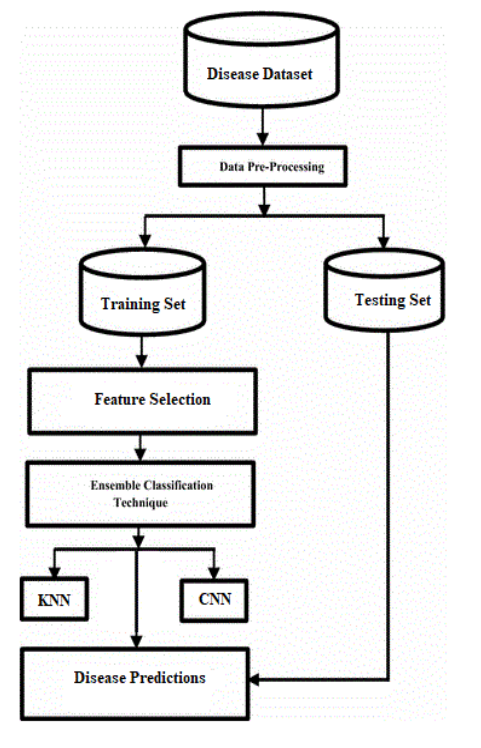
\includegraphics[scale=0.48]{1.png}
\end{center}
\end{frame}

\section{\textbf{Types}}

\begin{frame}{Types of Prediction System}
	\begin{itemize}
		\item Diabetes Prediction System
		\item Lung Cancer Prediction System
		\item Breast Cancer Prediction System
		\item Heart Disease Prediction System	
	\end{itemize}
\end{frame}



\section{\textbf{Diabetes Prediction System}}

\begin{frame}{Diabetes Prediction System}
	\begin{itemize}
		\item Internet
			
	\end{itemize}
\end{frame}

\section{\textbf{Lung Cancer Prediction System}}

\begin{frame}{Lung Cancer Prediction System}
\begin{itemize}
	\item Lung cancer is a harmful disease that causes a huge number of
	deaths globally. The primal encounter of lung cancer is
	necessary to decrease the mortality rate of patients. Thus it is a
	great challenge encountered by doctors and researchers to
	detect and diagnose lung cancer. Detection of lung cancer can
	be done by using medical images such as computed
	tomography, chest X-ray; MRI scans, etc., ML approaches
	recognize the main characteristics of complex lung cancer
	datasets. A CAD (Computer-Aided Diagnosis) was developed
	in the early 1980s to enhance the survival rate and efficiency
	that aid the doctors in interpreting medical images. Some of the
	machine learning algorithms that have a profound impact in
	health care are decision trees, linear regression, random forest,
	SVM, naive Bayes, K-nearest neighbors and so 
\end{itemize}
\end{frame}


\begin{frame}{Working Principle}
	\begin{itemize}
		\item A prototype lung cancer disease prediction system is
		developed using data mining classification techniques. 
		\item The system extracts hidden knowledge from a historical lung
		cancer disease database. 
		\item The most effective model to predict patients with Lung cancer disease appears to be
		Naïve Bayes followed by IF-THEN rule, Decision Trees and Neural Network.
		\item Decision Trees results are easier to read and interpret. 
		\item The drill through feature to access detailed patients’ profiles is only available in Decision Trees	
	\end{itemize}
\end{frame}

\section{\textbf{Heart Disease Prediction System}}

\begin{frame}{Heart Disease Prediction System}
	\begin{itemize}
		\item A prototype
	\end{itemize}
\end{frame}

\begin{frame}{Working Principle}
	\begin{itemize}
		\item For predicting heart attack, significantly 15 attributes are listed
		and with basic data mining technique other approaches e.g. ANN,Time Series, Clustering and Association Rules, soft computing approaches etc. can also be incorporated. 
		\item The outcome of predictive data mining technique on the same dataset reveals that
		Decision Tree outperforms and some time Bayesian classification is having similar accuracy as of decision tree but other predictive methods like KNN, Neural Networks, Classification based on clustering are not performing well.
		\item Decision Tree and Bayesian Classification further improves after applying genetic algorithm to reduce the actual data size to get the optimal subset of attribute sufficient for heart disease prediction.
	\end{itemize}
\end{frame}
\end{document}
